\chapter{Nalaganje podatkov}
\label{ch:nalaganje-podatkov}

Podatke, s katerimi smo delali do sedaj, smo dobili skupaj s programom Orange. Orange lahko bere tudi druge formate v obliki preglednic, npr. z vejico ali tabulatorjem ločene datoteke in Excelove preglednice. Pripravimo podatke (s šolskimi predmeti in ocenami) v Excelu in jih shranimo na računalnik.

V Orangeu podatke naložimo z gradnikom \widget{File}.

\begin{figure*}[h]
    \centering
    \newcommand{\excel}{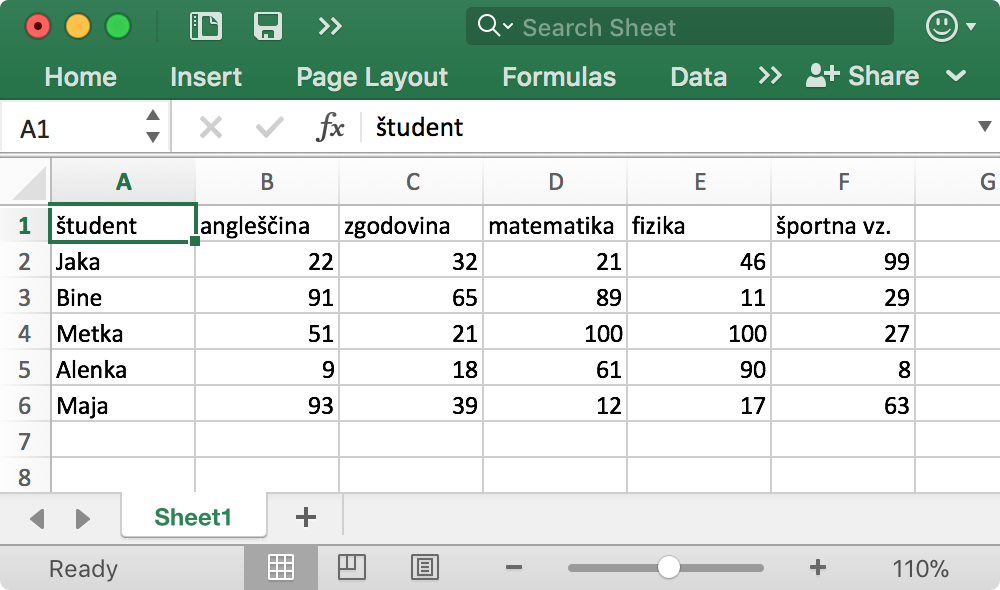
\includegraphics[scale=0.6]{excel.png}}
    \newcommand{\file}{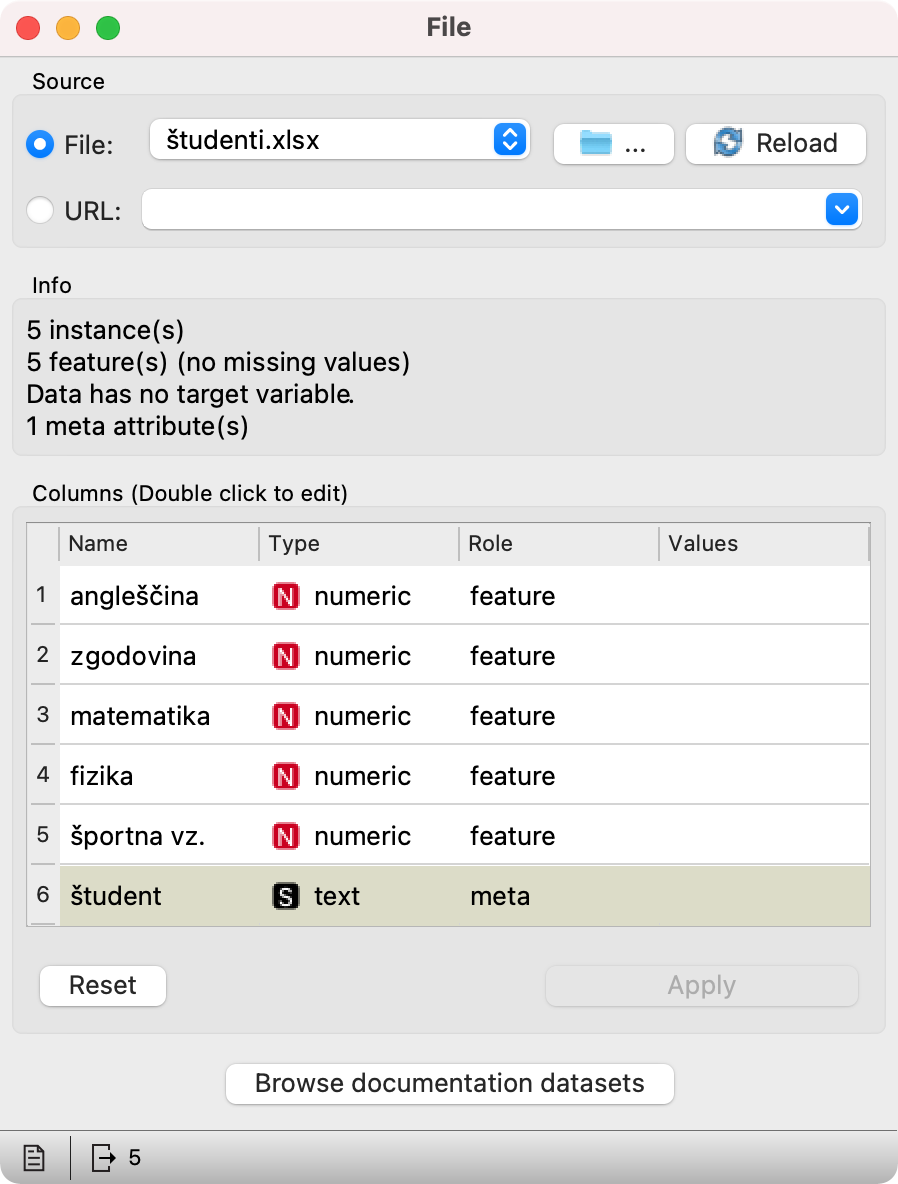
\includegraphics[scale=0.6]{file.png}}
    \infinitewidthbox{
    \stackinset{r}{-0.35\linewidth}{t}{+0.3\linewidth}{\file}{\excel}\hspace{6cm}
    }
\end{figure*}

\newpage

Orange je pravilno uganil, da so imena študentov besede in da je ta stolpec v podatkih nekaj posebnega - ponudi zgolj dodatne informacije in z njim ne delamo računskih operacij. Vsi ostali stolpci imajo številske vrednosti.
Vedno je koristno preveriti, če je Orange pravilno prebral podatke. Gradnik File povežemo z gradnikom Data Table,

\begin{figure}[h]
    \centering
    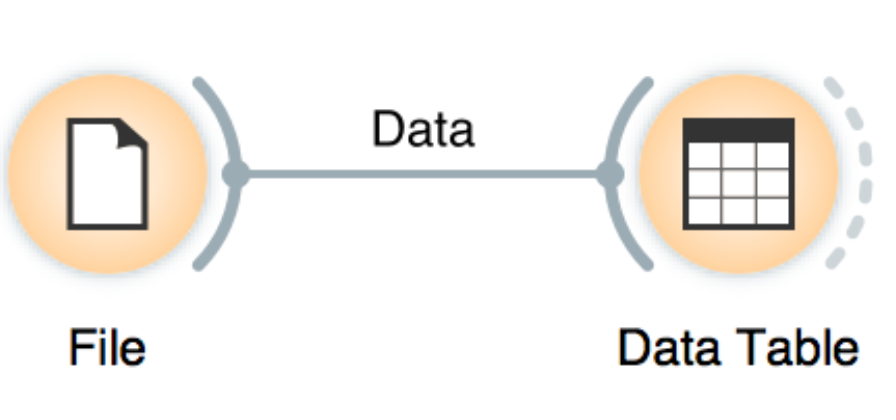
\includegraphics[width=0.5\textwidth]{workflow.png}
    \caption{$\;$}
\end{figure}

in dvakrat kliknemo na Data Table, da podatke prikažemo v preglednici.

\begin{figure*}[h]
    \centering
    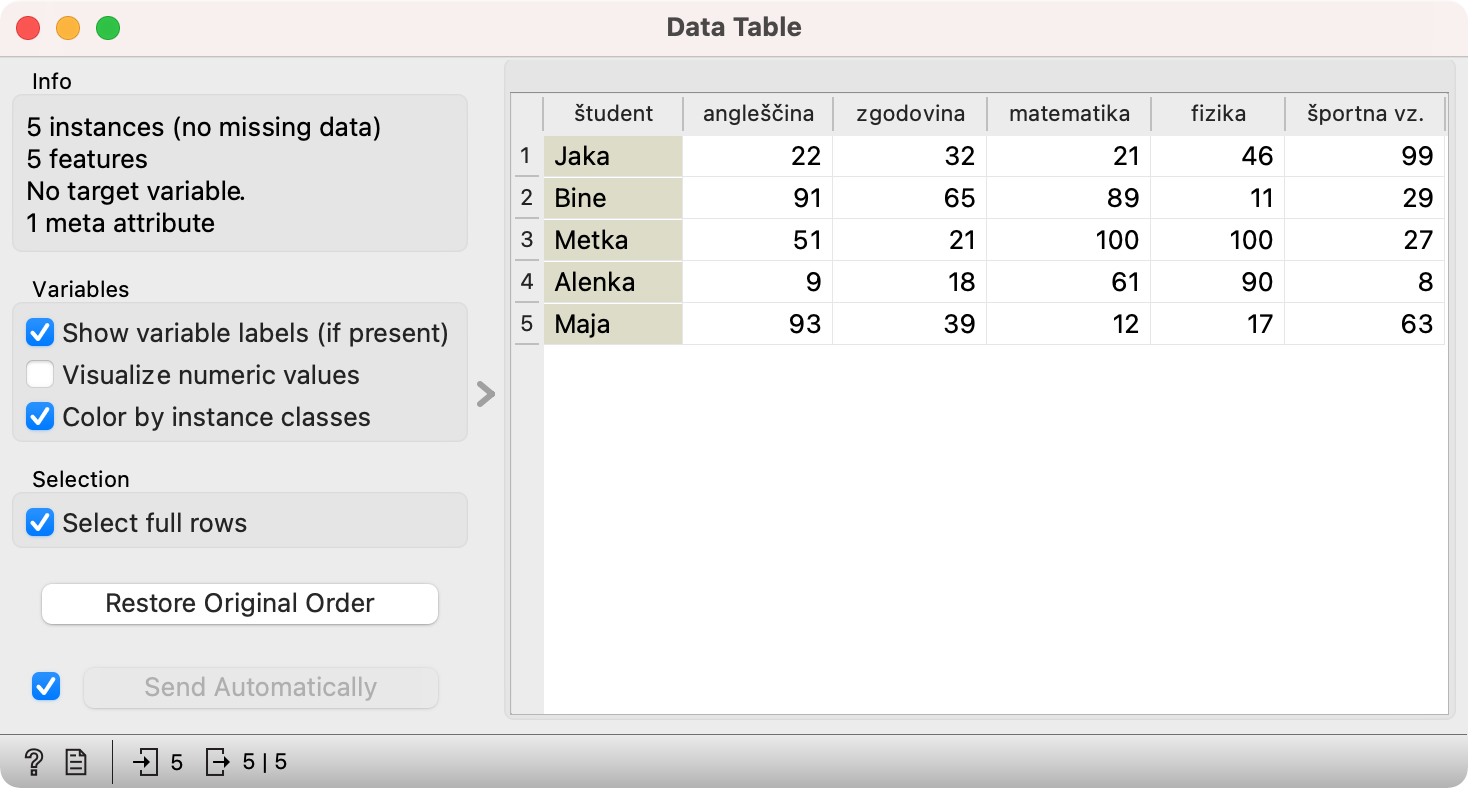
\includegraphics[width=0.8\textwidth]{data-table.png}
    \caption{$\;$}  % empty caption for correct figure placement
\end{figure*}

Odlično, vse je tako, kot mora biti.

Uporabimo lahko tudi Google Sheets, prosto dostopen spletni urejevalnik preglednic. Takrat, namesto nalaganja datoteke z računalnika, vnesemo spletno povezavo do dokumenta v vrstico URL v gradniku File.

Nalaganje in oblikovanje podatkov je široka tema. Definiramo lahko tip in vrsto stolpca, dodamo, da je stolpec povezava do slike, itd. Ampak dovolj zaenkrat. Če bi radi izvedeli več, poglejte dokumentacijo o nalaganju podakov ali video na to temo.